\documentclass[12pt]{article}
\usepackage{multicol,caption}
\setlength{\columnsep}{0.48cm}
\title{\textbf {Research Paper: DTL Assignment 5}}
\author{Amaan Jamdar}

\usepackage{geometry}
\usepackage{ragged2e}
\usepackage{graphicx}
\usepackage{tabularx}
\geometry{ a4paper, total= {170mm, 257mm}, left=20mm, top=20mm,}
\newenvironment{Figure}
  {\par\medskip\noindent\minipage{\linewidth}}
  {\endminipage\par\medskip}


\begin{document}
\maketitle
\clearpage

\begin{multicols*}{2}


\textbf{{\it  Abstract} - Computer
networks have become increasingly ubiquitous. In today's world, a computer network is much more than a collection of
interconnected devices. Computer networks are a
system of interconnected computers for the purpose of
sharing digital information. The computer network
enables to analyze, organize and disseminate the
information that is essential to profitability. The rise of
intranets and internets is the important aspect of
computer networking. Intranets and internets are private
business networks that are based on internet
technology. The businesses are currently implementing
intranets at a breakneck pace and for one reason only,
an intranet enables a business to collect, manage and
disseminate information more quickly and easily than
ever before. Many businesses are implementing
intranets simply to remain competitive; business that
delay is likely to see their competition outdistance
them. In this article we are presenting the basic
concepts of networking.\\ \\
\textit{Keywords: Linux, Windows, Mac, UI, Architecture, File
Management, Security}} \\


\section*{I. Introduction}
\indent \indent Networking supports communication between
two or more programs running on physically distant
machines. A computer network is a collection of
computers, which are in some way connected such that
they can exchange data between themselves and other
computers on the network. A network is created when
two or more computers are connected to share
information and resources. A set of computers
exchanging information by common conventions called
protocols over communication media. A computer
network is simply computers wired together in a way
that lets them share data and/or devices such as hard
drives, CD-ROMs, fax-modems, printers, etc \cite{2}. A
computer network is an interconnected collection of
autonomous computers where interconnected means
that the computers can exchange information and
autonomous means that no computer can start, stop or
control another computer connected to the network. Fig
1 gives an example of a network in a school comprising
of local area network or LAN connecting computers with each other, the internet, and various servers \cite{4}.\\

\begin{Figure}
 \centering
 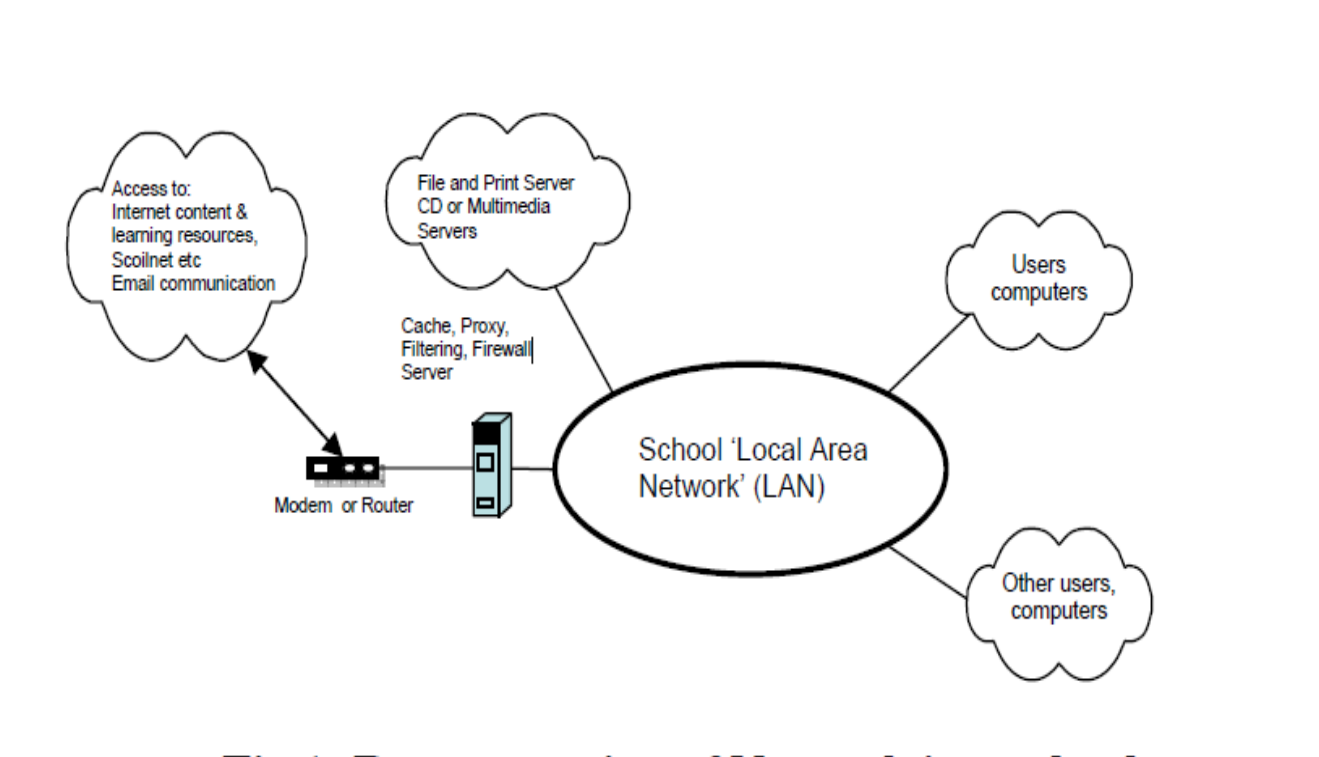
\includegraphics[width=\linewidth]{networkrepresent.png}
 \captionof{figure}{Representation of Network in a school}
\end{Figure}

\section*{II. Types Of Network Configuration}
\indent \indent Broadly speaking, there are two types of
network configuration, peer-to-peer networks and
client/server networks.

\subsection*{A. Peer-to-peer networks}
\indent \indent Peer-to-peer networks are more commonly
implemented where less than ten computers are
involved and where strict security is not necessary. All
computers have same status, hence the term "peer", and
they communicate with each other on an equal footing.
Files can be shared across the network and all the
computers on the network can share devices such as
printers or scanners, which are connected to any one
computer.Fig 2 represents how the computers are
connected in a peer-to-peer networks \cite{4}.

\begin{Figure}
 \centering
 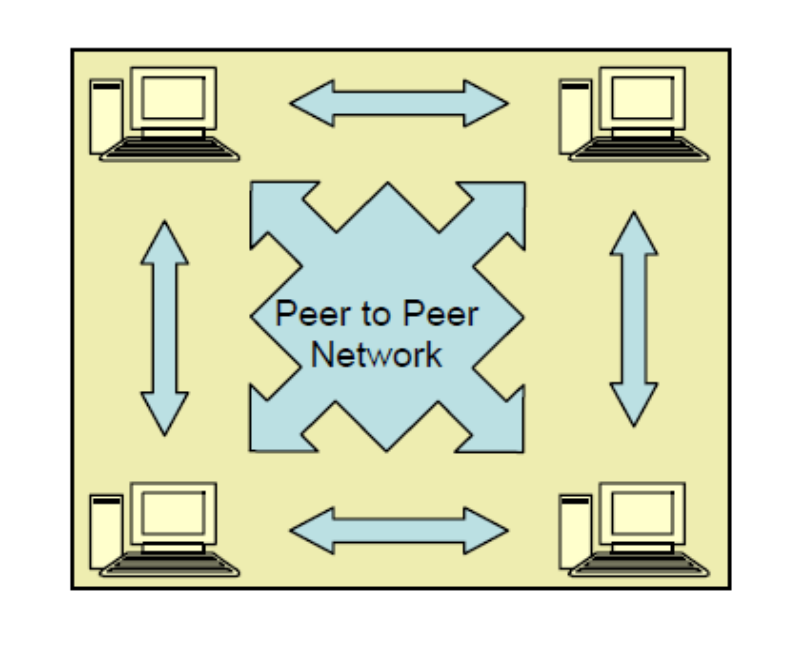
\includegraphics[width=\linewidth]{peer.png}
 \captionof{figure}{Peer to Peer networking}
\end{Figure}

\subsection*{B. Client/server networks}
\indent \indent Client/server networks are more suitable for
larger networks. A central computer, or "server", acts as
the storage location for files and applications shared on
the network. Usually the server is higher than an
average performance computer. The server also controls
the network access of the other computers which are
referred to as the "client" computers. Only the network
administrator will have access rights to the server while
others cannot. Others can only use the client computers.
Fig 3 represents how the computers are connected in a
client/server network \cite{4}.

\begin{Figure}
 \centering
 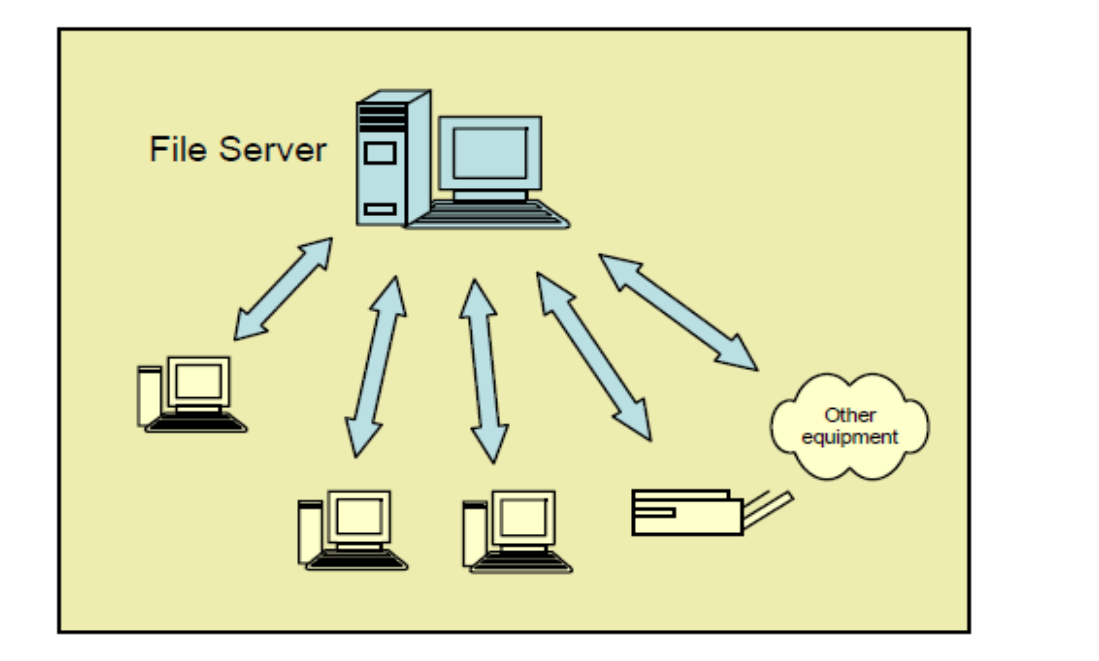
\includegraphics[width=\linewidth]{client.png}
 \captionof{figure}{Client Server Networking}
\end{Figure}

\section*{III. COMPONENTS OF A NETWORK}
A Computer network comprises the following components:
\begin{itemize}
  \item A minimum of at least two computers
  \item Cables that connect the computers each other,
although wireless communication is becoming
more common.
  \item A network interface device on each computer
(this is called a network interface card or NIC).
  \item A "switch" used to switch the data from one
point to another. Hubs are outdated.
  \item Network operating system software \cite{4}.
\end{itemize}

\section*{IV. Types of network}
The network can be divided into geographical
areas and fall into these major categories.
\begin{itemize}
  \item Local Area Network (LANs).
  \item Wide Area Network (WANs).
  \item Metropolitan Area Network (MANs).
  \item Wireless networks.
\end{itemize}

\subsection*{A. Local Area Network}
\indent \indent A LAN is generally confined to a specific
location, such as floor, building or some other small area. By being confined it is possible in most cases to
use only one transmission medium (cabling). This
technology is less expensive to implement than WAN
because you are keeping all of your expenses to a small
area, and generally you can obtain higher speed. They
are widely used to connect personal computers and
workstations in offices and factories to share the
resources. Traditional LANs runs at a speed of 10 to
100 mbps have low delay and make very few errors.
Never LANs may operate at higher speed up to 100
mbps.

\subsubsection*{1) Common Physical Topologies}
Physical and logical topologies can take several
forms. The most common and the most important for
understanding the Ethernet and Token Ring topologies
are:
\begin{itemize}
  \item Bus topology
  \item Ring topology
  \item Star topology
  \item Mesh topology
  \item Cellular topology
\end{itemize}

\subparagraph{a) Bus topology:}
\indent A bus physical topology is one in which all
devices connect to a common shared cable. A physical
bus topology network typically uses one long cable
called a backbone computers (workstation and servers)
are attached directly to the backbone using Terrestrial
microwave-connectors. The backbone is terminated at
both ends to remove the signal from the wire after it has
passed all devices. The bus topology is the first used
topology to connect the computers in a network. This is
the oldest form of topologies. This is a failure model.
Most bus topologies allow electric or electro-magnetic
signals to travel in both directions. A LAN with BUS
topology is represented in Fig 4.

\begin{Figure}
 \centering
 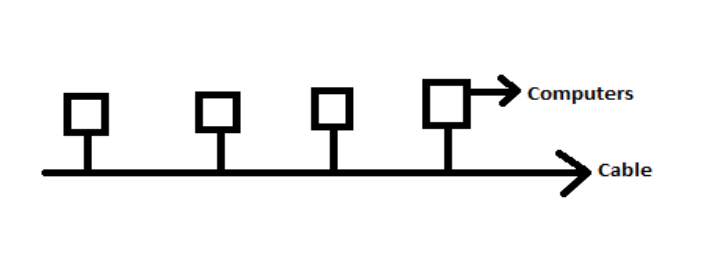
\includegraphics[width=\linewidth]{bus.png}
 \captionof{figure}{LAN with bus topology}
\end{Figure}

\subparagraph{b) Ring topology:}
\indent Ring topologies are wired in a circle. Each node
is connected to its neighbors or either side, passes
around the ring in one direction only. Each device
incorporates a receiver and a transmitter and serves as a
repeater that passes the signal to the next device in the
ring. Because the signal is regenerated at each device, signal degeneration is low. After some period of time
the RING topology came into existence. To avoid the
disadvantages of BUS topology, the RING topology is
invented. But this is also a failure model. Ring
topologies are ideally suited for token passing access
methods. The token gets passed around the ring, and
only the node that holds the token can transmit data.
Ring topologies are quite rare. A LAN with RING
topology is represented in Fig 5.

\begin{Figure}
 \centering
 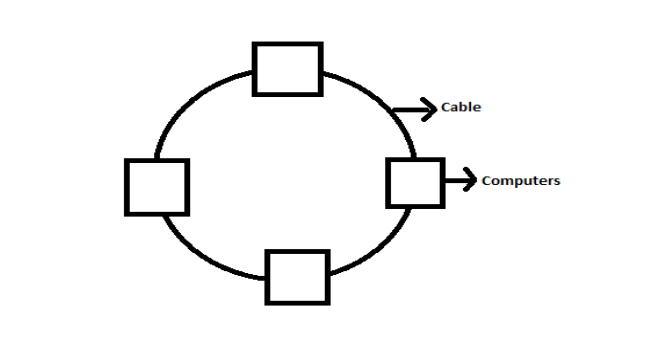
\includegraphics[width=\linewidth]{ring.png}
 \captionof{figure}{LAN with ring topology}
\end{Figure}

\subparagraph{c) Star topology:}
\indent Star topologies use a central device with drop
cables extending in all directions. Each networked
device is connected via a point-to-point link to the
central device called a hub or multiport repeater or
switch. Additionally, star topologies can be nested
within other stars to form tree or hierarchical network
topologies. In star topology, electrical or
electromagnetic signals travel from the networked
device, up its drop cable, to the switch, from there the
signal is sent to other network. To avoid the
disadvantages of BUS topology and RING topology,
the STAR topology is invented. This is not a failure
model. But it is a standard model and now-a-days this
topology is commonly used everywhere. A LAN with
STAR topology is represented in Fig 6.

\begin{Figure}
 \centering
 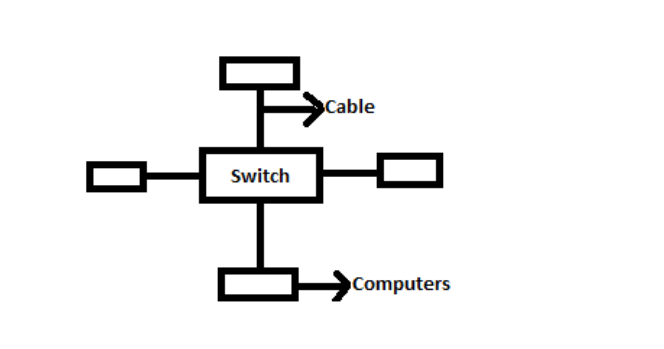
\includegraphics[width=\linewidth]{star.png}
 \captionof{figure}{LAN with star topology}
\end{Figure}

\subparagraph{d) Mesh topology}
\indent A mesh network has a point-to-point connection
between every device in the network. Because each device requires an interface for every other device on
the network, mesh topologies are not usually considered
practical. However, mesh networks are extremely fault
tolerant and each link provides guaranteed capacity.

\subparagraph{e) Cellular topology}
\indent A cellular topology combines wireless point-to-
point and multipoint strategies to divide a geographic
area into cells. Each cell represents the portion of the
total network area in which a specific connection
operates. Devices within the cell communicate with a
central station or switch. Switches are interconnected to
route data across the network and to provide the
complete network infrastructure. For example, devices
may roam from cell to cell while maintaining
connection to the network.

\subsection*{B. Wide Area Network}
\indent \indent A wide area network spans a large geographical
area, often a country or continent. It multiplies multiple
connected LANs that can be separated by any
geographical distance. In most WANs the network
contains numerous cables or telephone lines, each one
connection a pair of routers. If two routers that do not
share a cable nevertheless and wish to communicate,
they must do it indirectly. On personal computers we
are using modem to communicate indirectly with other
computer. WAN connecting two different networks is
represented in Fig 7.

\begin{Figure}
 \centering
 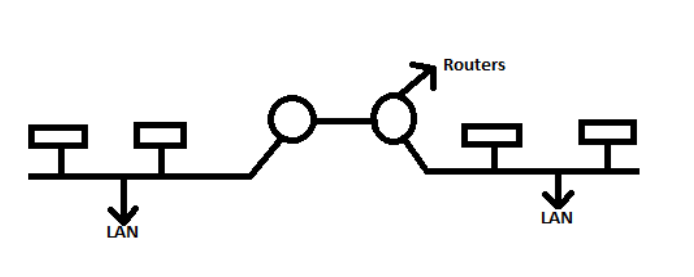
\includegraphics[width=\linewidth]{wan.png}
 \captionof{figure}{WAN connecting two different networks}
\end{Figure}

\subsection*{C. Metropolitan Area Network}
\indent \indent Metropolitan Area Network is basically a
bigger version of LAN and normally uses same
technology. It might cover a group of nearby corporate
offices or a city and might be either private or public.
On the other hand, MAN is network running throughout
a metropolitan area such as a backbone for a phone
service carrier. A MAN just has one or two cables and
does not contain switching elements.

\subsection*{D. Wireless Networks}
\indent \indent Mobile computers such as notebook computers,
laptops are the fastest growing segment of computer
industry. Users want to connect this machine to their office LANs to see the data when they are out from the
office, since the wired connection is not possible we
have to use wireless networks.

For e.g. on aircraft single router will maintain a
radio link with some other router on ground, changing
routers as it flies along this configuration is just a
traditional LAN, except that its connection to the
outside world happens to be a radio link instead of a
wired line.

\section*{V. COMMUNICATION LINKS}
Various types and forms of communication
medium are:
\begin{itemize}
  \item Fiber-optic cable.
  \item Twisted-pair copper wire.
  \item Coaxial cable.
  \item Wireless local-area links.
  \item Satellite channel \cite{3}.
\end{itemize}

\section*{VI. INTERNET PROTOCOL (IP)}
To solve the scaling problem with Ethernet, and
to allow support for other types of LANs and point-to-
point links as well, the Internet Protocol was developed.
To support universal connectivity, IP provides a global
mechanism for addressing and routing, so that packets
can actually be delivered from any host to any other
host. IP addresses (for the most common version 4,
which we denote IPv4) are 4 bytes (32 bits), \cite{6} and are
part of the IP header that generally follows the Ethernet
header. The Ethernet header only stays with a packet
for one hop; the IP header stays with the packet for its
entire journey across the Internet. An essential feature
of IPv4 addresses is that they can be divided into a
“network” part and a “host” part \cite{5}. There are different
types of classes in IPv4 and their ranges are shown in
Table 1.\\

\textbf{Table: 1 Range and types of classes} \\

\begin{noindent}
\begin{tabularx}{3.3in}{|X|X|}
\hline
Class & Addres Range\\ \hline
\RaggedRight{Class A} & \RaggedRight{0 to 126}\\
\hline
\RaggedRight{Class B} & \RaggedRight{128 to 191}\\
\hline
\RaggedRight{Class C} & \RaggedRight{192 to 223}\\
\hline
\RaggedRight{Class D} & \RaggedRight{224 to 239}\\
\hline
\RaggedRight{Class E} & \RaggedRight{240 to 254}\\
\hline
\end{tabularx} \\\\
\end{noindent}

Range 127 is reserved for the loopback or
localhost, for example, 127.0.0.1 is the common
loopback address. Range 255.255.255.255 broadcasts to
all hosts on the local network [9].


\section*{VII. OPEN SYSTEMS INTERCONNECTION(OSI) MODEL}
n 1977 the International Organization for
Standardization, or ISO, founded the Open Systems
Interconnection model, or OSI, a process for creation of
new network standards. OSI represented an attempt at
the creation of networking standards independent of any
individual government. The OSI model is today perhaps
best known for its seven-layer networking model.
Those seven layers of the OSI model and their purpose
are stated in Table 2. OSI has its own version of IP and
TCP. The IP equivalent is CLNP, the Connection Less
Network Protocol, although OSI also defines a
connection oriented protocol CMNS. The TCP
equivalent is TP4.\\

\textbf{Table: 2 Layers of OSI model and their purpose} \\

\begin{noindent}
\begin{tabularx}{3.3in}{|X|X|}
\hline
Layer & Purpose\\ \hline
\RaggedRight{Physical} & \RaggedRight{Network Interface Card, wire and so
on.}\\
\hline
\RaggedRight{Data Link} & \RaggedRight{Error checking, manages link
control, communication with cards.}\\
\hline
\RaggedRight{Network} & \RaggedRight{Addressing, traffic, switching}\\
\hline
\RaggedRight{Transport} & \RaggedRight{Handles network transmission}\\
\hline
\RaggedRight{Session} & \RaggedRight{Establishes rules for
communication, determines
synchronization.}\\
\hline
\RaggedRight{Presentation} & \RaggedRight{Translator between application and
others, redirector, encryption,
compression.}\\
\hline
\RaggedRight{Application} & \RaggedRight{Interface to network services.}\\
\hline
\end{tabularx} 
\end{noindent}


\section*{Conclusion}
Computer communication, it seems, will
become a much more useful networking tool when
large numbers of people with similar interests acquire
access to the technology. Though it can expedite the
formation of new interpersonal networks by
overcoming the space and time barriers faced by
traditional networking techniques, it still requires a
great deal of concentrated effort and resources to get the
people to use it. This problem should become
increasingly minimized over the coming years as the
technological innovations become more diffused
throughout society \cite{8}.
\end{multicols*}

\begin{thebibliography}{}
\bibitem{1} Cherita L. Corbett, Raheem A. Beyah, John A.
Copeland, Using Active Scanning to Identify
Wireless NICs, in: Proceedings of the 7th IEEE
Workshop on Information Assurance, U.S. Military
Academy, West Point, NY, 21-23 June 2006.
\bibitem{2} Pranab Kumar Chakravarty, Computer Networking
Technologies and Application to IT Enabled
Services.
\bibitem{3} Antonio Carzaniga, Basic concepts in Computer
Networking, September 19, 2014.
\bibitem{4} TeodoraBakardjieva, Introduction toComputer
Networking.
\bibitem{5} Peter L. Dordal, An Introduction to Computer
Networks, Release 1.8.07, June 16, 2015.
\bibitem{6} Bob Dickerson, Computer Networks, January
2005.
\bibitem{7} Russell Anthony Tantillo, Network Security
through Open Source Intrusion Detection Systems,
May 2012.
\bibitem{8} http://web.net/~robrien/papers/mpconclusion.html
\bibitem{9} http://www.computerhope.com/jargon/i/ip.htm



\end{thebibliography}

\end{document}

